%%%%%%%%%%%%%%%%%%%%%%%%%%%%%%%%%%%%%%%%%%%%%%%%%%%%%%%%%%%
% Tau
%%%%%%%%%%%%%%%%%%%%%%%%%%%%%%%%%%%%%%%%%%%%%%%%%%%%%%%%%%%

\documentclass[9pt,a4paper,twocolumn,twoside]{tau-class/tau}
\usepackage[english]{babel}
\usepackage{lipsum}
\usepackage[utf8]{inputenc}
\usepackage{pgfplots}
\usepackage{tikz}
\usetikzlibrary{angles, quotes, decorations.markings}
\pgfplotsset{compat=1.18}
\usepackage{xcolor}

%\usepackage{siunitx}

% Immagini come pdf
\usepackage{import}
\usepackage{xifthen}
\usepackage{pdfpages}
\usepackage{transparent}
\usepackage{hyperref}

\newcommand{\incfig}[1]{%
	\import{./img/}{#1.pdf_tex}
}

% Preambolo per tikz
\tikzset{midarrow1/.style = {postaction=decorate, decoration={markings,mark=at position .8 with \arrow{stealth}}}}
\tikzset{midarrow2/.style = {postaction=decorate, decoration={markings,mark=at position .4 with \arrow{stealth}}}}
\tikzset{midarrow/.style={midarrow1, midarrow2}}
\definecolor{lust}{rgb}{0.9, 0.13, 0.13}
\definecolor{richelectricblue}{rgb}{0.03, 0.57, 0.82}


% Preambolo documento
\journalname{Torino, 26 Aprile 2025}
\title{Esperienza di laboratorio: Spettroscopio}


\author[b,c,3]{Mattia Benna, Federico Cesari, Matteo Herz}


\professor{Università di Torino - Corso di Laurea in Fisica}


\institution{Unito, Fisica}
\theday{26 aprile, 2025}
\course{Esperimentazioni 2}


%----------------------------------------------------------
% ABSTRACT AND KEYWORDS
%----------------------------------------------------------

\begin{abstract}
L'esperimento ha permesso di approfondire i principi della dispersione ottica e di validare l'uso dello spettroscopio per l'analisi spettrale, evidenziando le differenze tra gli spettri di emissione del sodio e del mercurio. Abbiamo ricavato l'andamento dell'indice di rifrazione \(n\) del materiale del prisma in funzione della lunghezza d'onda \(\lambda\) della luce emessa ponendoci in condizione di deviazione minima.
\end{abstract}

%----------------------------------------------------------

%\keywords{spettroscopio}

%----------------------------------------------------------

\begin{document}
		
    \maketitle 
    \thispagestyle{firststyle} 
    \tauabstract
    % \tableofcontents
    % \linenumbers 
%----------------------------------------------------------

\section{Introduzione}
Lo studio degli spettri di emissione e assorbimento è fondamentale per comprendere la struttura della materia e le interazioni tra luce e atomi. Questo esperimento, condotto con uno spettroscopio a reticolo, permette di misurare le lunghezze d’onda delle righe spettrali emesse da lampade a vapori di sodio (Na) e mercurio (Hg), fornendo dati essenziali per analizzare proprietà ottiche come l’indice di rifrazione in funzione di $\lambda$. Tali misure sono rilevanti non solo per la fisica atomica, dove gli spettri rivelano livelli energetici quantizzati, ma anche per applicazioni pratiche, dalla calibrazione di strumenti ottici all’astronomia, dove l’analisi spettrale è usata per determinare la composizione chimica di stelle e galassie.

\section{Nozioni teoriche}
\subsection*{Dispersione del prisma}
La dispersione della luce attraverso un prisma è governata dalla legge di Snell e dalla geometria del sistema. In particolare, nel caso del prisma l’angolo di deviazione minima $D$ è legato all’indice di rifrazione $n$ e all’angolo al vertice $\alpha$ dalla formula:

\begin{equation}
n = \frac{\sin\left(\frac{D + \alpha}{2}\right)}{\sin\left(\frac{\alpha}{2}\right)}
\end{equation}

\noindent La condizione di deviazione minima si ottiene quando il percorso del raggio luminoso attraverso il prisma è simmetrico, ovvero quando l'angolo di incidenza e l'angolo di emergenza sono uguali.

Inoltre $n$ dipende a sua volta dalla lunghezza d'onda $\lambda$ attraverso la relazione empirica di Cauchy:
\begin{equation}
n(\lambda) = A + \frac{B}{\lambda^2}
\end{equation}

\subsection*{Diffrazione da reticolo}
Lo spettroscopio a reticolo sfrutta invece il fenomeno dell'interferenza multipla. Per un reticolo di diffrazione con passo $d$, la posizione angolare $\theta$ delle righe spettrali è determinata dalla condizione di interferenza costruttiva:

\begin{equation}
d\sin\vartheta = m\lambda \quad (m = 0, \pm 1, \pm 2, \dots)
\end{equation}

dove:
\begin{itemize}
\item $d$ è la distanza tra le fenditure del reticolo
\item $m$ è l'ordine di diffrazione
\item $\lambda$ è la lunghezza d'onda della luce
\item $\vartheta$ è l'angolo a cui si osserva il massimo di interferenza
\end{itemize}

Per $m=0$ si ha il massimo centrale, mentre gli ordini $m=\pm1$ corrispondono ai primi spettri diffratti. %La dispersione angolare aumenta con l'ordine $m$, permettendo di risolvere meglio righe vicine in lunghezza d'onda.


\section{Apparato e procedura sperimentale}
Sono stati utilizzati due dispositivi di dispersione: un prisma equilatero (\(\alpha = 60^\circ\)) e un reticolo di diffrazione con passo \(p = 3\times 10^{-6} m\). Questi sono posizionati al centro dello spettroscopio su una basetta rotante.
Lo spettroscopio è dotato di due cannocchiali, uno collimatore, che convoglia la luce contro il dispositivo posizionato sulla basetta, e un oculare, attraverso il quale guarda l'osservatore. Il cannocchiale oculare è mobile lungo un nonio circolare che permette di misurare la posizione angolare di quest'ultimo.

\begin{figure}[H]
    \centering
    \footnotesize
    \incfig{spettroscopio_prisma}
    \caption{Apparato sperimentale: spettroscopio}
\end{figure}

La prima misura effettuata, senza ancora utilizzare prisma o reticolo, è stata la direzione del raggio incidente. Con la fenditura quasi completamente chiusa determiniamo la posizione angolare della riga generata dalla luce della lampada attraverso la fenditura. 

Abbiamo quindi posizionato il prisma al centro della basetta rotante in condizione di deviazione minima. La luce emessa dalla lampada a vapori di sodio è stata diretta nella fenditura regolabile e convogliata dal collimatore fino al prisma. Il prisma ha disperso la luce generando uno spettro visibile. Abbiamo osservato le diverse righe spettrali ruotando l'oculare e per ogni riga osservata è stato registrato l'angolo di deviazione, corrispondente alla posizione angolare della riga. Abbiamo poi ripetuto le misure per lo spettro generato dalla lampada a vapori di mercurio.

Successivamente, il prisma è stato sostituito con il reticolo di diffrazione, verificando che questo risultasse il più perpendicolare possibile al raggio incidente. Nel cannocchiale oculare sono apparse le righe spettrali di diffrazione e di queste abbiamo registrato la posizione angolare dei massimi +1,+2\footnote{Poiché non è stato possibile eseguire un  confronto col suo corrispettivo simmetrico i valori associati al massimo +2 non sono stati utilizzati nell'analisi dati} e -1.


\section{Analisi dati e discussione}
Conclusa la presa dati abbiamo due set distinti, il primo ricavato dallo spettro di emissione della lampada al sodio:

\begin{table}[H]
            \centering
            \begin{tabular}{cccc}
                \toprule
                \(n_\text{Na}\) & \(\delta_n\) & \(\lambda\) (nm) & \(\delta_\lambda\) (nm) \\
                \midrule
                1.6168 & 0.0002	& 605	& 2 \\
                1.6192 & 0.0002	& 579	& 2 \\
                1.6206 & 0.0002	& 560	& 2 \\
                \bottomrule   
            \end{tabular}
		\caption{Presa dati da lampada al sodio}
            %\tabletext{Note: se c'è qualcosa da far notare: quì!}
\end{table}
e il secondo ricavato dallo spettro di emissione della lampada al mercurio:
\begin{table}[H]
            \centering
            \begin{tabular}{cccc}
                \toprule
                \(n_\text{Hg}\) & \(\delta_n\) & \(\lambda\) (nm) & \(\delta_\lambda\) (nm) \\
                \midrule
                1.6158 &	0.0002	&618	&8 \\
                1.6167 &	0.0002	&606	&9 \\
                1.6173 &	0.0002	&603	&7 \\
                1.6189 &	0.0002	&586	&7 \\
                1.6197 &	0.0002	&570	&9 \\
                1.6199 &	0.0002	&568	&9 \\
                1.6230 &	0.0002	&537	&8 \\
                1.6303 &	0.0002	&488&	8 \\
                1.6306 &	0.0002	&484&	7 \\
                1.6368 &	0.0002	&444&	10 \\
                1.6502 &	0.0002	&401&	6 \\
                1.6512 &	0.0002	&397&	4 \\
                \bottomrule  
            \end{tabular}
            \caption{Presa dati da lampada al mercurio}
            %\tabletext{Note: se c'è qualcosa da far notare: quì!}
\end{table}
Notiamo che l'incertezza relativa su \(\lambda\) per la lampada al sodio risulta essere, in media, di un ordine di grandezza inferiore rispetto a quella per la lampada al mercurio (\(\delta_{\text{rel Na}} \approx 0.15\%\) e \(\delta_{\text{rel Hg}} \approx 1.5\%\)).
Ciò deriva dal fatto che si sono ottenuti dati con una dispersione minore (più precisi) per le lunghezze d'onda estratte dalla lampada al sodio rispetto a quelle estratte dalla lampada al mercurio.  Ecco perché nel grafico sono visibili alcuni punti con barre di errore significativamente più piccole rispetto alle altre (si veda ad esempio il 2° punto da sinistra nel Dettaglio A). Questo è stato causato da un disallineamento accidentale del reticolo che ha reso quest'ultimo non perfettamente perpendicolare al raggio incidente. Ciò ha portato a variare leggermente i valori di \(\lambda\) dei massimi -1 e +1, determinando quindi una semidispersione maggiore. ciononostante, l'andamento atteso dai dati non è stato influenzato in modo significativo.


%Questo potrebbe essere giustificato da due fattori in particolare: in primo luogo, essendo la lampada al mercurio più intensa come luce, ci ha costretto a restringere la fenditura di entrata del collimatore, perdendo intensità luminosa e dunque risoluzione, a discapito però di una migliore separazione delle righe spettrali più ravvicinate. In secondo luogo, avendo effettuato le misure per la lampada al mercurio successivamente a quelle del sodio, non è da trascurare una possibile imprecisione dovuta alla stanchezza dell'occhio dell'osservatore, tenendo anche conto delle condizioni di scarsa illuminazione presenti in laboratorio durante la presa dati.  

Una volta ottenute le lunghezze d'onda delle rispettive righe di emissione tramite l'utilizzo del reticolo di diffrazione e i diversi valori dell'indice di rifrazione \(n\) del materiale del prisma, abbiamo confrontato l'andamento di \(n\) in funzione di \(\lambda\) con quello teorico dato dall'approssimazione di Cauchy; relazione valida per descrivere la dispersione normale in materiali trasparenti nello spettro del visibile. Per ogni riga di emissione abbiamo misurato la posizione angolare dei 3 massimi di ordine +1, -1, +2, con l'aspettativa di ottenere valori di \(\lambda\) coerenti tra loro. Purtroppo non è stato possibile osservare ogni colore (riga di emissione) per ogni ordine di massimo, visto il decrescere dell'intensità luminosa all'aumentare di \(\theta\).

Avendo a disposizione solo due misure per ogni riga spettrale (una per il massimo +1 e una per il -1) si è deciso di associare la semidispersione massima come incertezza sulla lunghezza d'onda. La semidispersione restituisce una stima conservativa ma secondo noi anche più realistica dell’errore. In questo modo si evita in parte di sottostimare l’incertezza reale, soprattutto in un esperimento con così pochi dati, per cui non è accurato propagare gli errori gaussianamente. La scelta ci è quindi sembrata coerente con l’obiettivo di rappresentare in modo trasparente i limiti del metodo sperimentale adottato.

Il valore di \(\lambda\)  è stato banalmente ottenuto come la media della coppia di dati raccolti.
Di seguito mostriamo il grafico dei valori ottenuti, evidenziandone l'accordo con l'andamento teorico atteso:
\begin{figure}[H]
    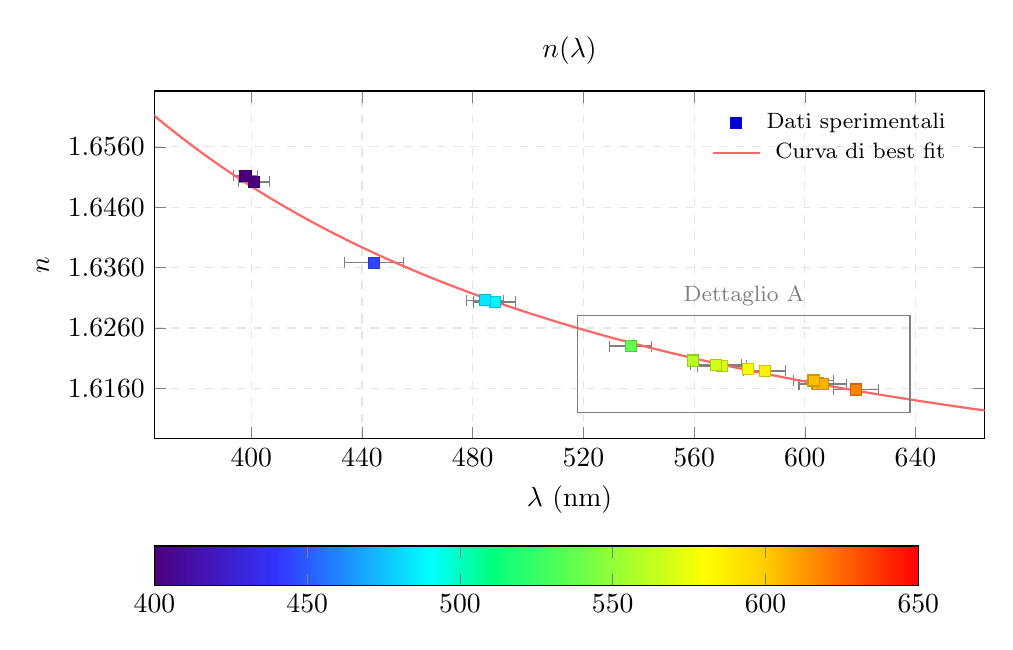
\begin{tikzpicture}
        \begin{axis}[
            title={\(n(\lambda)\)},
            width=\linewidth,
            height=6cm,
            xlabel={\(\lambda\) (nm)},
            ylabel={\(n\)},
            grid=both,
            grid style={dashed, gray!20},
            ytick={1.6160,1.6260,1.6360,1.6460,1.6560},
            yticklabels={1.6160,1.6260,1.6360,1.6460,1.6560},
            xtick={400, 440, 480, 520,560, 600, 640},
            xticklabels={400, 440, 480, 520,560, 600, 640},
            xmin=365, xmax=665,
            legend pos=north east,
            legend style={
                draw=none,
                fill=none,
                text opacity=1,
                font=\footnotesize,
                cells={anchor=east}
            },
            colormap={visiblespectrum}{
                rgb(400)=(0.3,0,0.5)   % violet (corrected wavelength)
                rgb(440)=(0.2,0.2,1)   % blue
                rgb(490)=(0,1,1)     % cyan
                rgb(510)=(0,1,0.5)   % green
                rgb(580)=(1,1,0)     % yellow
                rgb(600)=(1,0.8,0)   % orange
                rgb(650)=(1,0,0)     % red
            },
            point meta min=400,
            point meta max=650
            ]

            % Dati principali con colori dello spettro
            \addplot+ [
            scatter,
            only marks,
            mark=square*,
            scatter src=x,
            mark size=2,
            visualization depends on={\thisrow{yerr}\as\perror},
            visualization depends on={\thisrow{xerr}\as\xerror},
            error bars/.cd,
            x dir=both, x explicit,
            y dir=both, y explicit,
            error bar style={line width=0.5pt, solid, black!50}
            ] table [
            x=x,
            y=y,
            x error=xerr,
            y error=yerr,
            ] {
                y     yerr   x       xerr
                1.6168	0.0002	604.59	1.35
                1.6192	0.0002	579.42	1.42
                1.6206	0.0002	559.67	1.42	
                1.6158	0.0002	618.41	8.10
                1.6167	0.0002	606.50	8.58
                1.6173	0.0002	603.16	7.15
                1.6189	0.0002	585.51	7.64
                1.6197	0.0002	570.11	8.77
                1.6199	0.0002	567.93	9.19
                1.6230	0.0002	537.14	7.58	
                1.6303	0.0002	487.91	7.65
                1.6306	0.0002	484.43	6.65
                1.6368	0.0002	444.34	10.51
                1.6502	0.0002	400.94	5.53
                1.6512	0.0002	397.91	4.31
            };
            \addlegendentry{Dati sperimentali}

            \addplot[
            red!60,
            thick,
            domain=340:750,
            samples=200
            ] {
                1.5913 + 9304/x^2
            };
            \addlegendentry{Curva di best fit}

            \draw[gray]
            (axis cs:518,1.612) rectangle
            (axis cs:638,1.628);

            \node[gray,above, align=center, font=\footnotesize] at (axis cs:578,1.628)
            {Dettaglio A};

            % Barra dei colori con spettro visibile
            \pgfplotsset{
                colorbar horizontal,
                colorbar style={
                    xtick={400,450,500,550,600,650},
                    width=0.8\linewidth,
                    xlabel style={yshift=-0.5cm},
                    colormap name=visiblespectrum
                }
            }
        \end{axis}
    \end{tikzpicture}
    \centering
    \caption{Unione dei dati ricavati con la lampada al sodio e di quelli ricavati con la lampada al mercurio. I punti sono colorati secondo lo spettro visibile corrispondente alla loro lunghezza d'onda, da 400 nm (viola) a 650 nm (rosso). La regione delimitata (Dettaglio A) verrà analizzata separatamente nella figura successiva.}
\end{figure}

\begin{figure}[H]
    \centering
    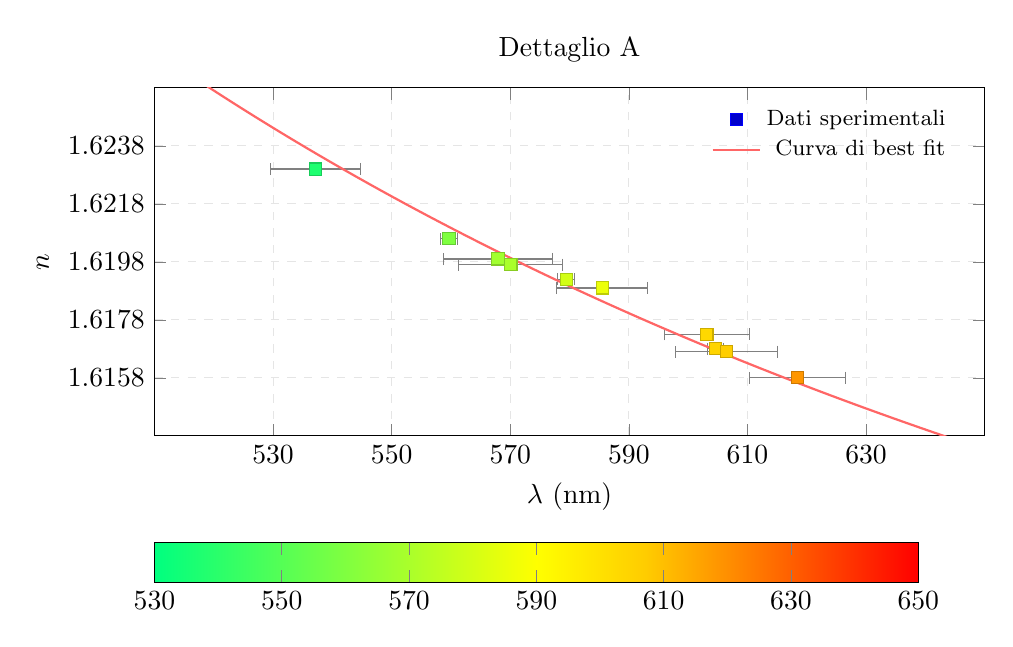
\begin{tikzpicture}
        \begin{axis}[
            title={Dettaglio A},
            width=\linewidth,
            height=6cm,
            xlabel={\(\lambda\) (nm)},
            ylabel={\(n\)},
            grid=both,
            grid style={dashed, gray!20},
            ytick={1.6158,1.6178,1.6198,1.6218,1.6238},
            yticklabels={1.6158,1.6178,1.6198,1.6218,1.6238},
            xtick={530,550,570,590,610,630},
            xticklabels={530,550,570,590,610,630},
            xmin=510, xmax=650,
            ymin=1.6138, ymax=1.6258,
            legend pos=north east,
            legend style={
                draw=none,
                fill=none,
                text opacity=1,
                font=\footnotesize,
                cells={anchor=east}
            },
            colormap={visiblespectrum}{
                rgb(510)=(0,1,0.5)   % green
                rgb(580)=(1,1,0)     % yellow
                rgb(600)=(1,0.8,0)   % orange
                rgb(650)=(1,0,0)     % red
            },
            point meta min=530,
            point meta max=650
            ]

            % Dati principali con colori dello spettro
            \addplot+ [
            scatter,
            only marks,
            mark=square*,
            scatter src=x,
            mark size=2.2,
            visualization depends on={\thisrow{yerr}\as\perror},
            visualization depends on={\thisrow{xerr}\as\xerror},
            error bars/.cd,
            x dir=both, x explicit,
            y dir=both, y explicit,
            error bar style={line width=0.5pt, solid, black!50}
            ] table [
            x=x,
            y=y,
            x error=xerr,
            y error=yerr,
            ] {
                y     yerr   x       xerr
                1.6168	0.0002	604.59	1.35
                1.6192	0.0002	579.42	1.42
                1.6206	0.0002	559.67	1.42	
                1.6158	0.0002	618.41	8.10
                1.6167	0.0002	606.50	8.58
                1.6173	0.0002	603.16	7.15
                1.6189	0.0002	585.51	7.64
                1.6197	0.0002	570.11	8.77
                1.6199	0.0002	567.93	9.19
                1.6230	0.0002	537.14	7.58
            };
            \addlegendentry{Dati sperimentali}

            \addplot[
            red!60,
            thick,
            domain=340:750,
            samples=200
            ] {
                1.5913 + 9304/x^2
            };
            \addlegendentry{Curva di best fit}

            % Barra dei colori con spettro visibile
            \pgfplotsset{
                colorbar horizontal,
                colorbar style={
                    xtick={530,550,570,590,610,630,650},
                    width=0.8\linewidth,
                    xlabel style={yshift=-0.5cm},
                    colormap name=visiblespectrum
                }
            }
        \end{axis}
    \end{tikzpicture}
    \caption{Ingrandimento sul raggruppamento di misure con \(\lambda > 530\)nm.}
\end{figure}
%
\begin{table}[H]
            \centering
            \begin{tabular}{cc}
                \toprule
                $\chi^2$ & \(6.95\) \\
                $A$ & $1.5913 \pm 0.0001$ \\
                $B$ & $\;\;\;\;9304 \pm 66 \text{ nm}^2$\\
                \bottomrule   
            \end{tabular}
            \caption{Parametri ottenuti dal fit con la curva di Cauchy}
\end{table}

Quanto ottenuto attraverso la regressione dei dati conferma l'accordo della curva teorica descritta dalla legge di Cauchy con i dati ottenuti sperimentalmente. Il valore del $\chi^2$ ottenuto risulta ampiamente accettabile entro un livello di significatività del $5\%$ senza raggiungere un valore sospetto. %\\
 
%Se però ad un primo impatto visivo le barre d'errore ricavate per le lunghezze d'onda della lampada ai vapori di mercurio possono sembrare ampie, è giusto commentare e giustificare la scelta chi vi sta dietro. 
%E' stata infatti adottata la semidispersione come stima dell’incertezza sulle lunghezze d’onda, preferendola alla propagazione gaussiana degli errori per due motivi principali. Innanzitutto, il numero limitato di misurazioni ripetute per ciascuna riga spettrale (2-3 dati) rende meno significativa una stima puramente statistica, mentre la semidispersione fornisce un criterio "robusto" anche con pochi dati. In secondo luogo, le principali fonti di incertezza in questo esperimento come il posizionamento del reticolo, la messa a fuoco ed il rilevamento delle righe spettrali attraverso l’oculare, così come la lettura del goniometro, sono di natura sistematica o comunque difficili da quantificare singolarmente. 

%La semidispersione, riflettendo direttamente la variabilità osservata nei dati, può tener conto anche di questi fattori, restituendo una stima conservativa ma secondo noi anche più realistica dell’errore. Dunque, sebbene questo approccio porti a barre di errore più ampie rispetto alla propagazione gaussiana teorica, esso evita in parte di sottostimare l’incertezza reale, soprattutto in un esperimento con così pochi dati in cui tali fonti di errore possono dominare sulle fluttuazioni puramente casuali. La scelta ci è quindi sembrata coerente con l’obiettivo di rappresentare in modo trasparente i limiti del metodo sperimentale adottato.

%\color{red}{Commenti su barre di errore molto piccole visti i lambda molto vicini tra loro/possibile confronto con errori ottenuti con propagazione gaussiana mostrando che in entrambi i casi si ottiene un chi quadro accettabile, in modo da giustificare una non sovrastima degli errori.}

\section{Conclusioni}
L'esperimento condotto ha consentito di verificare empiricamente la relazione tra l'indice di rifrazione di un prisma e la lunghezza d'onda della luce, confermando i fenomeni della dispersione ottica e della diffrazione previsti teoricamente. Mediante l'utilizzo di uno spettroscopio in configurazione di deviazione minima e due lampade al sodio e al mercurio, sono stati determinati gli indici di rifrazione corrispondenti alle diverse righe spettrali e le lunghezze d'onda associate sono state stimate attraverso un reticolo di diffrazione, analizzando le righe dei primi due ordini.

Le discrepanze osservate tra i valori calcolati per le due lampade sono state attribuite a un errore sistematico, riconducibile a un probabile disallineamento del reticolo. Nonostante ciò, l'andamento del grafico ottenuto segue con accuratezza l'andamento dato dalla legge di Cauchy.



%----------------------------------------------------------

\printbibliography

%----------------------------------------------------------

\end{document}